\documentclass[12pt, a4paper, oneside, fontset=windows]{ctexart}
\usepackage{amsmath, amsthm, amssymb, appendix, bm, graphicx, hyperref, mathrsfs}

\title{\textbf{最优化第一次小组作业}}
\author{孙璇,付星桐,郅啸淇,林庭申}
\date{\today}
\linespread{1.5}
\usepackage{graphicx}
\usepackage{pythonhighlight}
\usepackage{float}
\lstset{
	%backgroundcolor=\color{red!50!green!50!blue!50},%代码块背景色为浅灰色
%	rulesepcolor= \color{gray}, %代码块边框颜色
	breaklines=true,  %代码过长则换行
	numbers=left, %行号在左侧显示
	numberstyle= \small,%行号字体
	%keywordstyle= \color{blue},%关键字颜色
	commentstyle=\color{gray}, %注释颜色
%	frame=shadowbox%用方框框住代码块
	frame=single,
	escapeinside=``    % 代码包含中文
}

\newtheorem{theorem}{定理}[section]
\newtheorem{definition}[theorem]{定义}
\newtheorem{lemma}[theorem]{引理}
\newtheorem{corollary}[theorem]{推论}
\newtheorem{example}[theorem]{例}
\newtheorem{proposition}[theorem]{命题}

\renewcommand{\abstractname}{\Large\textbf{摘要}}

\begin{document}
\pagestyle{empty}
\maketitle

\setcounter{page}{0}
\maketitle
\thispagestyle{empty}



\newpage
% 添加目录
\pagenumbering{Roman}
\setcounter{page}{1}
\tableofcontents
\newpage
\setcounter{page}{1}
\pagenumbering{arabic}

\newpage
\section*{作业:多元线性回归}
在回归分析中,如果有两个或两个以上的自变量,就称为多元回归。事实上,一种现象常常是与多个因素相联系的,由多个自变量的最优组合共同来预测或估计因变量,比只用一个自变量进行预测或估计更有效,更符合实际。因此多元线性回归比一元线性回归的实用意义更大

%$\underset{\mathbf x }{min}\frac{1}{2}\Vert \mathbf A \mathbf x +\mathbf b\Vert_2^{2}$

\section{方法简介}
\subsection{正规方程法}
$y(x_{1},x_{2},x_{3}......x_{n}) = w_{0} + w_{1}x_{1} + w_{2}x_{2}+...+w_{n}x_{n}$

$ = x^{T}*w$

上述是拟合函数的一般形式,其中第二行的 x = (x0,x1,x2...xn),w = (w0,w1...wn),上述是一组数据的表达式,例如有 m 个样本数据,那么 x 可以表示为 m*n 维矩阵,w 表示为 1*n 维矩阵。w 也就是 x 前的系数,取自weigh的首字母,有权重的含义。上述损失函数的公式可以写成如下形式。

$H=\sum_{i=0}^{n} (x_{i}^{T}w - y_{i})^{2}$


然后进行对 w 求导计算,令导数为0,最终整理结果为

$w = (x^{T}_{i}x)^{-1}x^{T}y$

相对于代数计算,这样更方便,而且更利于计算机编程。

\subsection{梯度下降法}
梯度下降法又称最速下降法,是求解无约束最优化问题的一种最常用的方法,在对损失函数最小化时经常使用。梯度下降法是一种迭代算法。选取适当的初值x(0),不断迭代,更新x的值,进行目标函数的极小化,直到收敛。由于负梯度方向时使函数值下降最快的方向,在迭代的每一步,以负梯度方向更新x的值,从而达到减少函数值的目的

梯度下降是用于找到可微函数的局部最小值的一阶迭代优化算法。为了使用梯度下降找到函数的局部最小值,我们采取与该数在当前点的梯度(或近似梯度)的负值成比例的步骤。
\subsubsection{固定步长法}
我们可以通过来控制每一步走的距离,以保证不要走的太快,错过了最低点(右图所示),同时也要保证收敛速度不要太慢

所以在选择大小的时候在梯度下降中是非常重要的,不能太大也不能太小

\subsubsection{后退线性搜索}
后退线性搜索是一种最常用的不精确搜索策略,如果当前步长无法满足需要,就把步长乘上$\beta$,达到步长后退的效果,为了保证结果,$\alpha$和$\beta$的选取也很重要
\section{数据集1}
数据集1包含以下四列:TV,Radio,Newspaper,Sales。本次研究目的为使用最小二乘法求解三种不同的广告方式投入(TV,Radio,Newspaper)对销量(Sales)的影响(多元线性回归)。
\subsection{正规方程法}
首先是使用正规方程法求解出来的回归系数和回归系数预测值和真实值的残差二范数
\begin{python}
    #方法1:最小二乘问题的解析解
    xa=((AT*A).I)*AT*(b.T)
    #求出预测值
    pre=A*xa
    print('解析解求得的系数:\n',xa)
    print('解析解求得的范数最小值:\n',1/2*np.linalg.norm(A*xa-b.T,ord=2))
\end{python}
\begin{python}
    解析解求得的系数:
    [[0.57647987]
    [0.39922791]
    [0.03226498]]
   解析解求得的范数最小值:
    0.4870182675954456
\end{python}

可以看到TV和Radio对于Sales的影响较大,而Newspaper的影响较小。

下图中红色直线即为正规方程法找到的最小范数。
\begin{figure}[H]
    \centering
    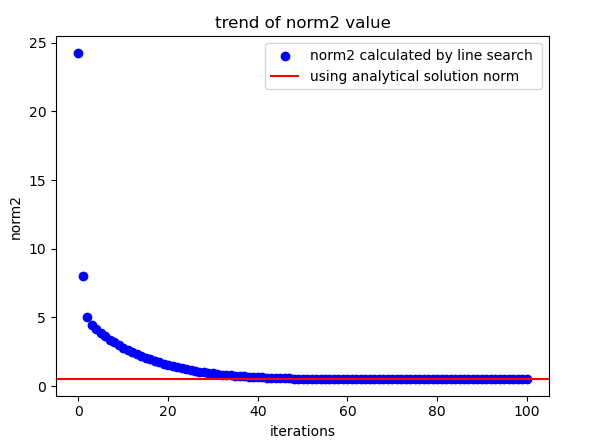
\includegraphics[width=10cm,height=8cm]{Analytical Solution Norm2.png}
    \caption{Iteration of Norm2:Analytical Solution}
\end{figure} 
\subsection{梯度下降法}
\subsubsection{固定步长法}
然后使用梯度下降法中的固定步长法寻找最小二乘法最小值,本次步长选取为$a1 = 0.01$
\begin{python}
    #方法2:固定步长
    #设定固定步长a1(切换不同步长真的很重要)
    a1=0.01
    #设定初始迭代点
    xf=np.matrix([[10],[10],[10]])
    #设置画布
    p=plt.figure(figsize=(14,14))
    ax1=p.add_subplot(2,2,1)
    x1=xf
    result=[]#用于存放得到的结果
    #开始进行迭代
    for j in range(1000):
        x1=x1-a1*AT*(A*x1-b.T)
        preg=pd.DataFrame(A*x1-b.T)
        norm=1/2*np.linalg.norm(preg,ord=2)
        if 1/2*np.linalg.norm(A*x1-b.T,ord=2)-1/2*np.linalg.norm(A*(x1-a1*AT*(A*x1-b.T))-b.T)<0.00001:#如果前后两值相差小于0.00001则达到停止条件
            break    
        result.append(norm)
    #设置画布横坐标
    label=[i for i in range(j)]
    print('使用固定步长法的迭代次数为:\n',j)
    print('使用固定步长法求得的范数最小时的系数(解)为:\n',x1)
    print('使用固定步长法求得的范数最小值:\n',1/2*np.linalg.norm(A*x1-b.T,ord=2))
    #作图
    plt.scatter(label,result,color='b')
    #plt.plot(x,1/2*np.linalg.norm(A*x-b.T,ord=2))
    plt.ylabel('norm2')
    plt.xlabel('')
\end{python}
\begin{python}
    使用固定步长法的时间为:
    21019500
   使用固定步长法的迭代次数为:
    101
   使用固定步长法求得的范数最小时的系数(解)为:
    [[0.57568831]
    [0.3964474 ]
    [0.03890155]]
   使用固定步长法求得的范数最小值:
    0.4871002366328933
\end{python}

从运行结果上看,本次下降速度较快,最终收敛结果和正规方程法所得系数基本一致。

从图像中看,蓝色散点图为固定步长法的迭代轨迹,固定步长法在四十次迭代左右即达到正规方程法的效果
\begin{figure}[H]
    \centering
    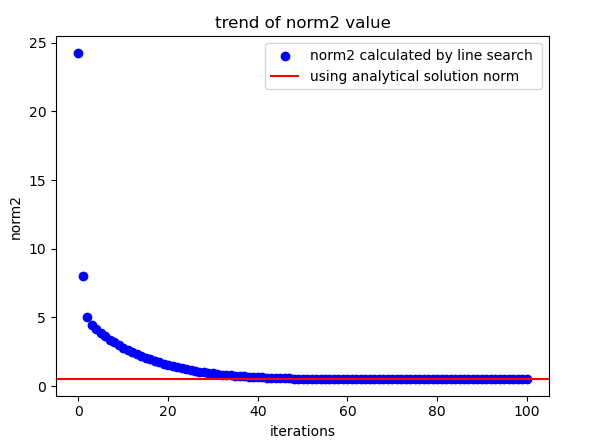
\includegraphics[width=10cm,height=8cm]{Analytical Solution Norm2.png}
    \caption{Iteration of Norm2:Line Search}
\end{figure}
\subsubsection{后退线性搜索}
\begin{python}
    #方法3:后退线性搜索
    #设置ba是α,bb是β和t
    ba=0.01
    bb=0.1
    t=1
    #设定初始迭代点
    xf2=np.matrix([[1],[1],[1]])
    x2=xf2
    cnt=0
    result2=[]
    while True:
        while 1/2*np.linalg.norm(A*(x2-t*AT*(A*x2-b.T))-b.T,ord=2)>1/2*np.linalg.norm(A*x2-b.T,ord=2)-ba*t*(AT*(A*x2-b.T)).T*(AT*(A*x2-b.T)):
            t=bb*t
        cnt+=1
        x2=x2-t*AT*(A*x2-b.T)
        result2.append(1/2*np.linalg.norm(A*x2-b.T,ord=2))
        if 1/2*np.linalg.norm(A*x2-b.T,ord=2)-1/2*np.linalg.norm(A*(x2-t*AT*(A*x2-b.T))-b.T)<0.00001:
            break
    print('使用后退搜索法的迭代次数为:\n',cnt)
    print('使用后退搜索法求出的系数(解)为:\n',x2)
    print('使用后退搜索法求出的范数最小值为:\n',1/2*np.linalg.norm(A*x2-b.T,ord=2))
    #同样设定横坐标
    label2=[i for i in range(cnt)]
    ax2=p.add_subplot(2,2,2)
    plt.scatter(label2,result2,color='y')
    plt.ylabel('norm2')
    
    ax3=p.add_subplot(2,2,3)
    plt.scatter(label,result,color='b')
    plt.scatter(label2,result2,color='y')
    plt.show()
\end{python}
\begin{python}
    使用后退搜索法的时间为:
 28025400
使用后退搜索法的迭代次数为:
 71
使用后退搜索法求出的系数(解)为:
 [[0.57571188]
 [0.39653196]
 [0.03870066]]
使用后退搜索法求出的范数最小值为:
 0.4870953474145896
\end{python}

根据运行结果,在$\alpha = 0.01$和$\beta = 0.1$的条件下,后退法得到的最终系数和最小范数结果基本一致。

从图像上可以看出来,在$\alpha = 0.01$和$\beta = 0.1$的条件下,后退法在迭代二十次左右即可收敛到正规方程法的结果。
\begin{figure}[H]
    \centering
    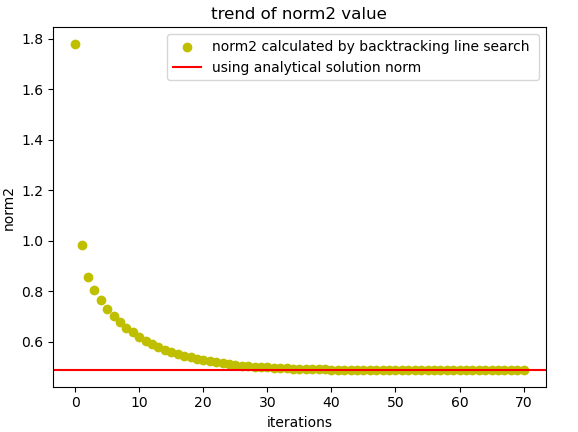
\includegraphics[width=10cm,height=8cm]{Backtracking Line Search.png}
    \caption{Iteration of Norm2:Backtracking Line Search}
\end{figure}
\subsubsection{两种方法对比}
\begin{figure}[H]
    \centering
    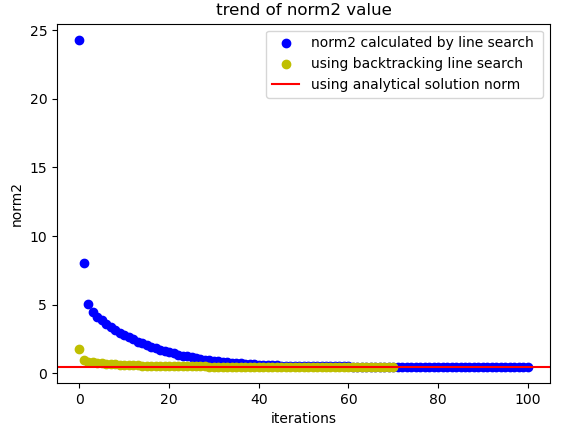
\includegraphics[width=10cm,height=8cm]{Overall Contrast.png}
    \caption{Iteration of Norm2:Overall Contrast}
\end{figure}
我们将两种方法得到的迭代曲线放在一起,可以看出两种方法的迭代次数上有一定的差异,但是最终都能很好的收敛到正规方程法的结果上。

两者的迭代次数和运行时间在本数据集中也差异不大,后退法在开始时步长较大,减少了迭代次数。
\end{document}